% !TeX TXS-program:bibliography = txs:///biber
\documentclass[unknownkeysallowed]{beamer}
\usetheme{UniKlu}
\usepackage[backend=biber,style=apa,sorting=nty, bibencoding=utf8]{biblatex}
\addbibresource{/home/donkarlo/Dropbox/projs/research/refs.bib}


\usepackage{xcolor}

\title{Help from the Sky: Leveraging UAVs for Disaster Management}
\author{Mohammad Rahmani}
\institute{Pervasive Computing Group}

\begin{document}
\begin{frame}
	\maketitle
\end{frame}

\begin{frame}{UAVs and Wireless Sensor Networks}
	Different kinds of Unnamed Aerial Networks (UAVs) can be used to enhance disaster management together with Wireless Sensor Networks (WSN) based on differed disaster types and stages. 
	\begin{figure}
		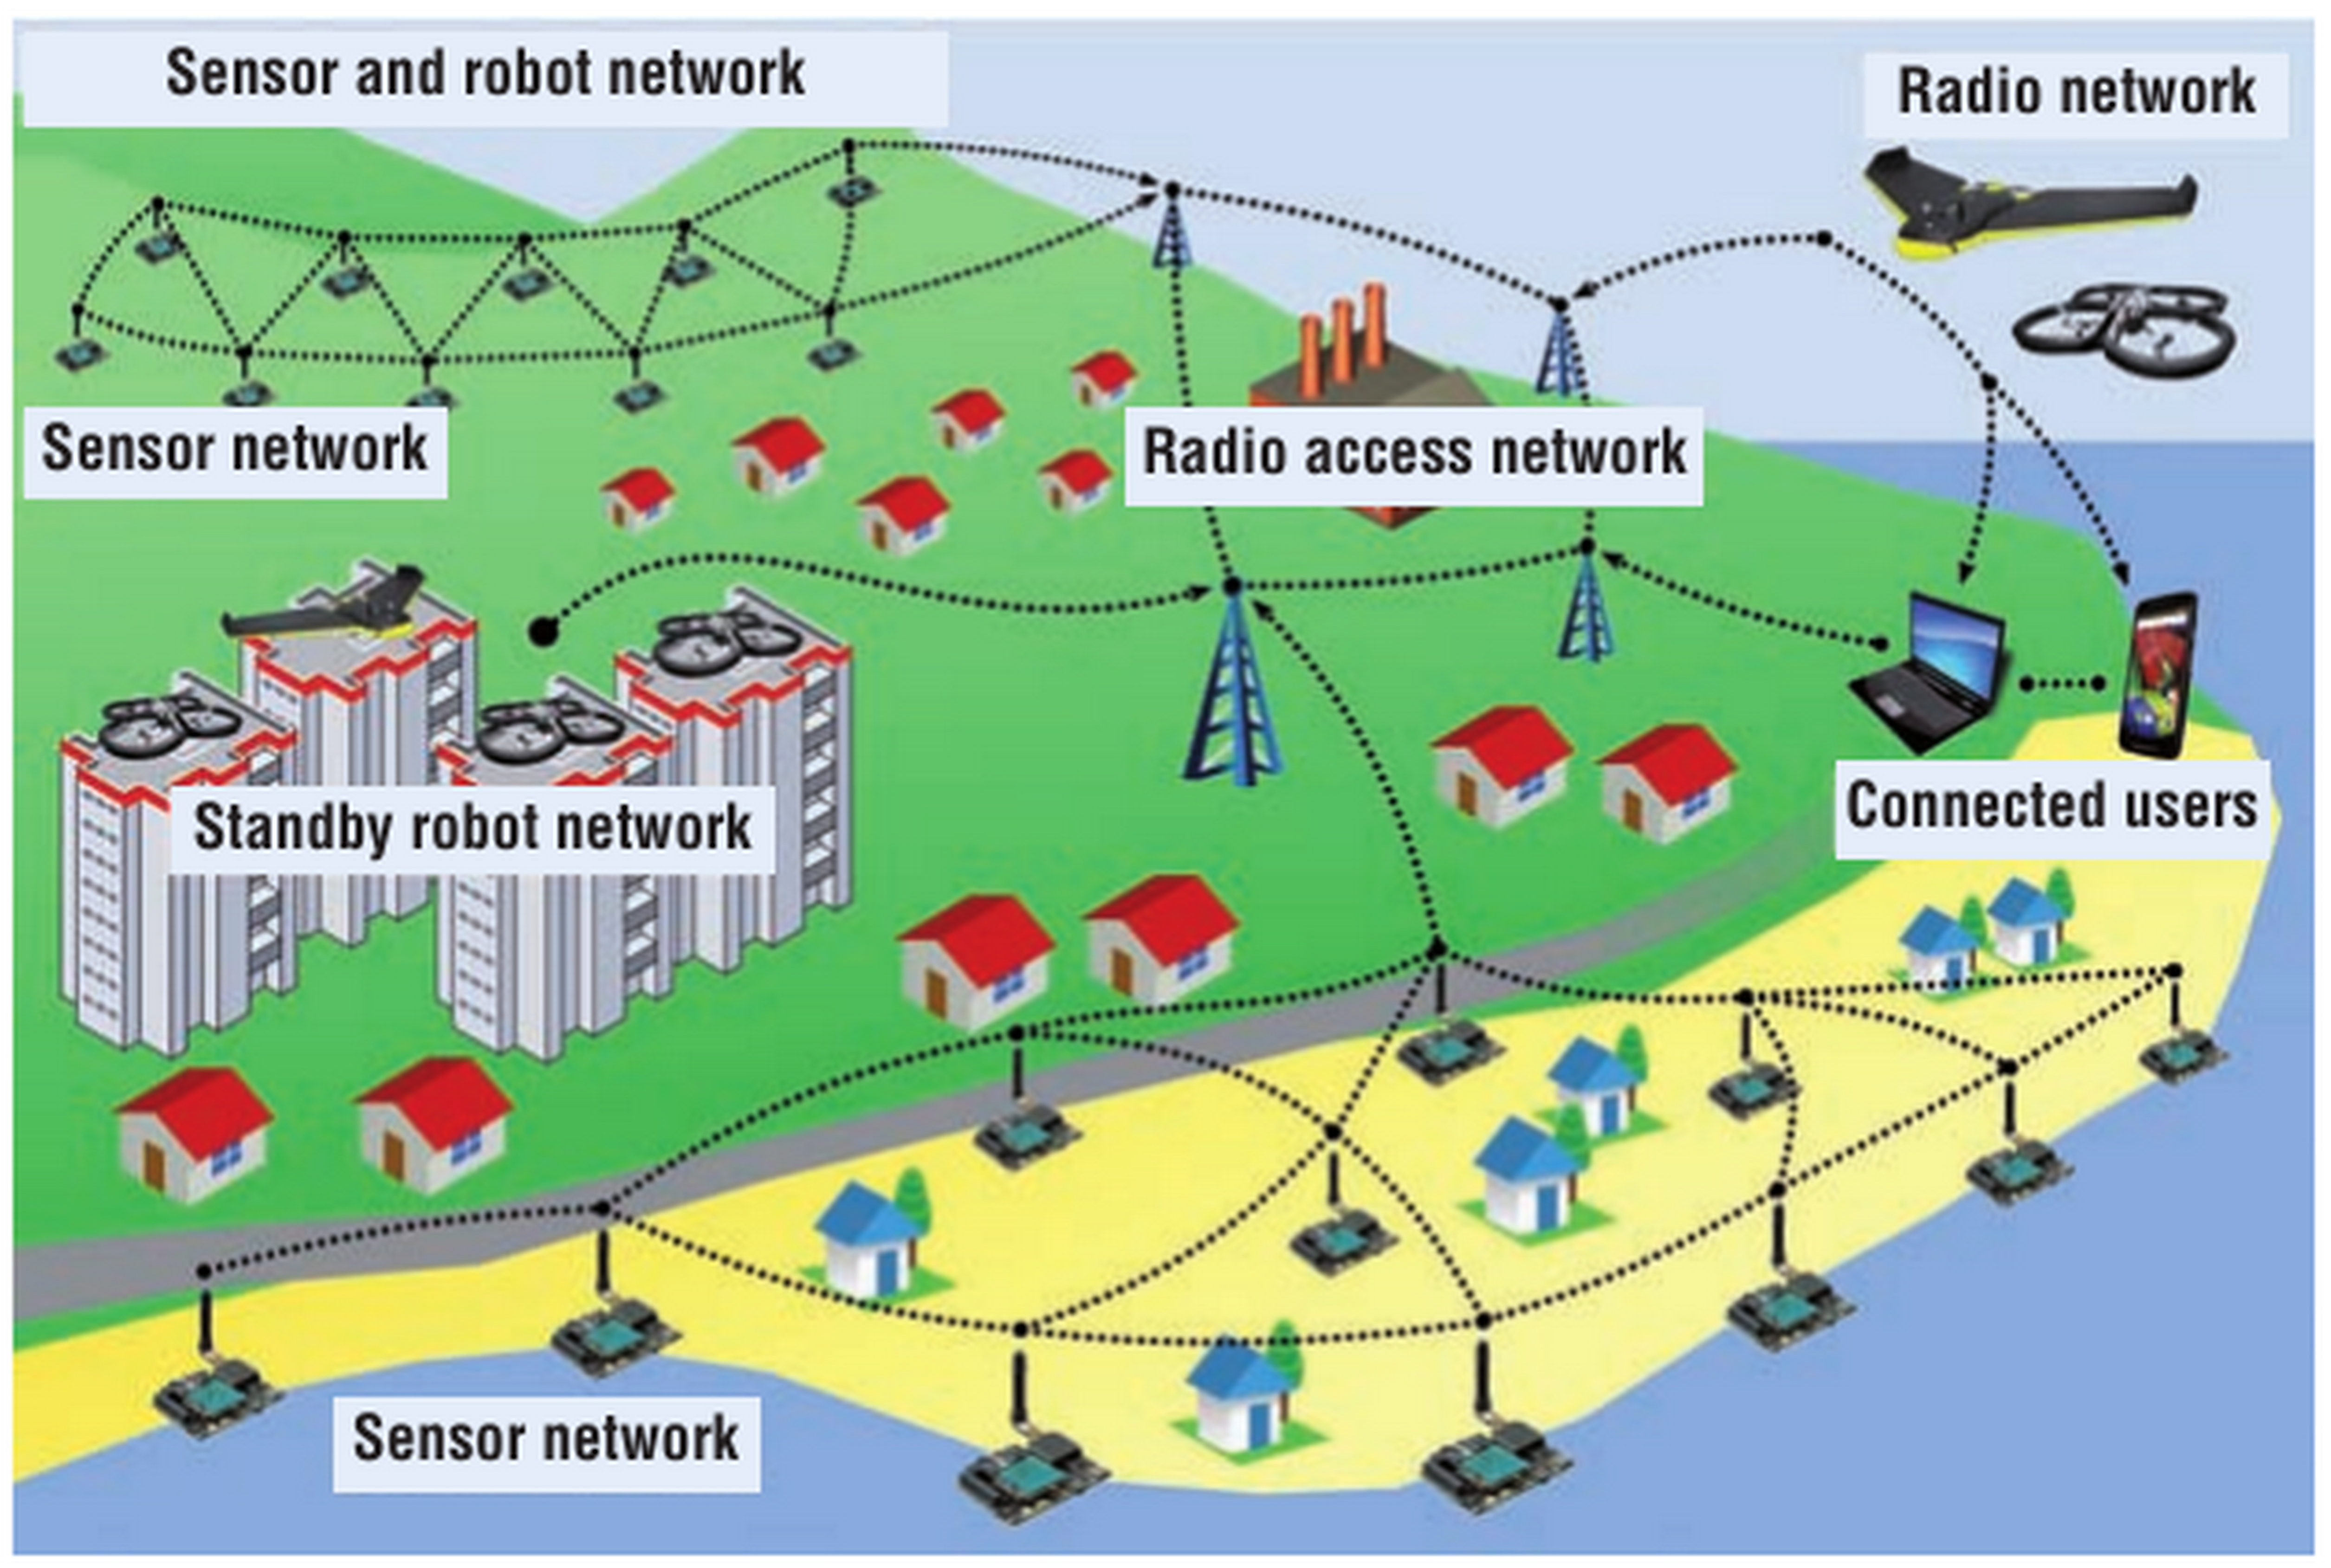
\includegraphics[scale=0.45]{uav-wsn.jpg}
	\end{figure}
\end{frame}

\begin{frame}{Applications of UAVs}
	\begin{itemize}
		\item Monitoring and forecasting and early warnings
		\item Disaster information fusion and sharing
		\item Situational awareness and logistic and evacuation support
		\item Standalone communication system
	\end{itemize}
\end{frame}

\begin{frame}{Applications of UAVs - 2}
	\begin{itemize}
		\item Search and Rescue (SAR) missions
		\item Damage assessment
		\item Media coverage
		\item Medical applications
		\item Infrastructure construction
	\end{itemize}
\end{frame}

\begin{frame}{Problems of using UAVs}
	\begin{itemize}
		\item Power supply limitation
		\item Unreliable communication channel
		\item Unexpected node failure
		\item Maximal physical load size
		\item Maneuverability in harsh conditions
	\end{itemize}
\end{frame}

\begin{frame}{Features of UAV networks}
	\begin{itemize}
		\item \textbf{Energy-effectiveness trade-offs}: They have small battery capacity so their network must be (sub)optimal
		\item \textbf{Dynamic topologies}: They have vulnerable localization abilities due to high impact of on-filed changes such as air drifts. As such error control approaches must be considered
		\item \textbf{Multi-objective downtime}: During downtime such as battery recharges questions such as keeping the same network with more redundancy or changing the topology should be answered. 
	\end{itemize}
\end{frame}

\begin{frame}{Different Types of UAVs}
	\begin{itemize}
		\item \textbf{Fixed Wings}: Large area coverage but expensive
	\end{itemize}
	
	\textbf{Rotary wings}: Can be sent exactly to critical spot
	\begin{itemize}
		\item \textbf{Helicopters}: Large payload delivery but expensive
		\item \textbf{Multi-rotor}: Low price but short flight duration
	\end{itemize}
\end{frame}

\begin{frame}{Tasks in Different stages of the Disasters}
	\begin{itemize}
		\item \textbf{Stage 1 (Preparedness)}: Early Warning System (EWS) for static threshold sensing and surveying by UAVs
		\item \textbf{Stage 2 (Assessment)}: Situational awareness and damage study
		\item \textbf{Stage 3 (Response)}: Supporting SAR missions - Building communication links for Radio Access Network  (RAN). Government related policy
	\end{itemize}
	\textbf{Main argument}: Static WSN is not sufficient and a dynamic topology supported by UAVs should be implemented for all the above stages. 
\end{frame}

\begin{frame}{Different Types of Disaster}
	\begin{itemize}
		\item \textbf{Type A}: Geophysical(earthquake) and hydrological(flash-floods)
		\item \textbf{Type B}: Climatological (Drought)
		\item \textbf{Type C}: Meteorological (Tropical storm)
	\end{itemize}
\end{frame}

\begin{frame}{Preparedness Stage for all Types}
	WSNs should be used but UAVs at this stage will have limited role. 
	\begin{itemize}
		\item Optimize WSN data acquisition and data analysis to assess the probability of future disaster occurrences, using UAVs as data mules
	\end{itemize}
\end{frame}

\begin{frame}{Assessment Stage}
	\begin{itemize}
		\item \textbf{Type A}: Assessment only by UAV: \textbf{Improvement}: Use heterogeneous UAV networks comprising fixed-wing UAVs to scan
the area and identify important points to be covered and surveyed by rotary-wing UAVs
		\item \textbf{Type B}: Assessment by UAV and parts of WSN which are still functional: \textbf{Improvement}:UAV network and WSN network can re-establish the partial connection losses
		\item \textbf{Type C}: Only WSN can be used for situational awareness: \textbf{Improvement}: fuse WSN and social media network data
	\end{itemize}
\end{frame}

\begin{frame}{Response/Recovery Stage}
	\begin{itemize}
		\item \textbf{Type A}: Only UAVs for SAR, monitoring and communication restoration: \textbf{Improvement}: Use special UAV sensors and actuators mounted on UAVs
		\item \textbf{Type B}: UAVs and WSN restore broken connectivity: \textbf{Improvement}: Maximal application of WSN data in UAVs for SAR
		\item \textbf{Type C}: Only WSN with integration of aerial surveys can be used for efficient decision support systems: \textbf{Improvement}: Use WSN to reconnect impaired UAV networks.
	\end{itemize}
\end{frame}

\begin{frame}{Open issues}
	For type A and B
	\begin{itemize}
		\item Creating and maintaining the information relay network.
		\item Supporting in-network data fusion
		\item Addressing handover issues
	\end{itemize}
\end{frame}

\begin{frame}{Open issues- 2}
	For Type C
	\begin{itemize}
		\item Develop specialize hardware for sever environmental conditions for UAVs
		\item Develop special software for controlling UAVs in sever conditions
	\end{itemize}
\end{frame}

\begin{frame}{Open issues- 3}
	General
	\begin{itemize}
		\item Automating network maintenance and UAV charging
		\item Increasing UAV network security and robustness
		\item Handling UAV failures
		\item Ensuring privacy and trust
	\end{itemize}
\end{frame}

\begin{frame}{Questions}
	Thanks a lot. Questions?
\end{frame}

\end{document}
